%
% skalar.tex -- Skalarprodukt
%
% (c) 2018 Prof Dr Andreas Müller, Hochschule Rapperswil
%
\section{Orthogonale Projektion und Skalarprodukt\label{section:ortho-skalar}}
\index{Skalarprodukt}
Abstand und Winkel spielen in der euklidischen Geometrie eine fundamentale
Rolle, die bisher eingeführten Elemente der Vektorgeometrie erlauben
jedoch noch nicht, Abstände oder Winkel zu berechnen.
Aus der elementaren Trigonometrie ist bekannt, dass der Schlüssel dazu
das Verständnis rechtwinkliger Dreiecke ist.
Der Kosinus eines Winkels ist das Verhältnis von Ankathete zu Hypothenuse.
De Ankathete ist aber auch die orthogonale Projektion der Hypothenuse
auf die Richtung der Ankathete.
Das Skalarprodukt soll daher aus der orthogonalen Projektion entwickelt
werden.

\subsection{Orthogonale Projektion\label{subsection:orthoproj}}
\index{orthogonale Projektion}
\index{Projektion!orthogonale|see{orthogonale Projektion}}
Zunächst möchten wir zeigen, dass sich Längen und Winkel berechnen
lassen, wenn man in der Lage ist, die Länge der orthogonalen Projektion
eines Vektors $\vec{v}$ auf jeden beliebigen anderen Vektor $\vec{u}$
zu berechnen.
\begin{figure}
\begin{center}
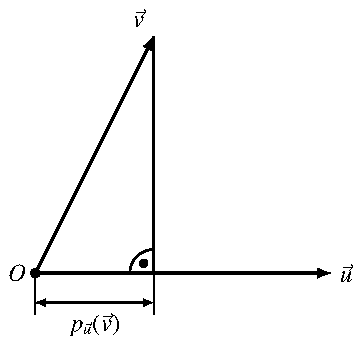
\includegraphics{4/images/projektion.pdf}
\end{center}
\caption{Orthogonale Projektion\label{orthproj}}
\end{figure}

Seien also $\vec u$, $\vec v$ zwei beliebige Vektoren wie in Abbildung~\ref{orthproj}, und $p_{\vec u}(\vec v)$
die Länge der Projektion des Vektors $\vec v$ auf $\vec u$.
Wir versehen diese Länge mit einem Vorzeichen, zeigt der auf $\vec u$
projizierte Vektor $\vec v$ in die gleiche Richtung wie $\vec u$
nehmen wir die Länge positiv, zeigt der projizierte Vektor in die
Gegenrichtung, ist $p_{\vec u}(\vec v)$ negativ.

Die Länge von $\vec v$ ist $p_{\vec v}(\vec v)$, und für den Winkel
$\alpha$ zwischen den beiden Vektoren ist
\begin{equation}
\cos \alpha = \frac{p_{\vec u}(\vec v)}{p_{\vec v}{\vec v}}.
\label{zwischenwinkel}
\end{equation}
Offenbar ist die Länge der Projektion die grundlegendere Grösse,
aus der man die anderen Konzepte ableiten kann.
Etwas ungünstig ist an dieser Projektion nur, dass die beiden Vektoren nicht
symmetrisch eingehen.
\begin{figure}
\centering
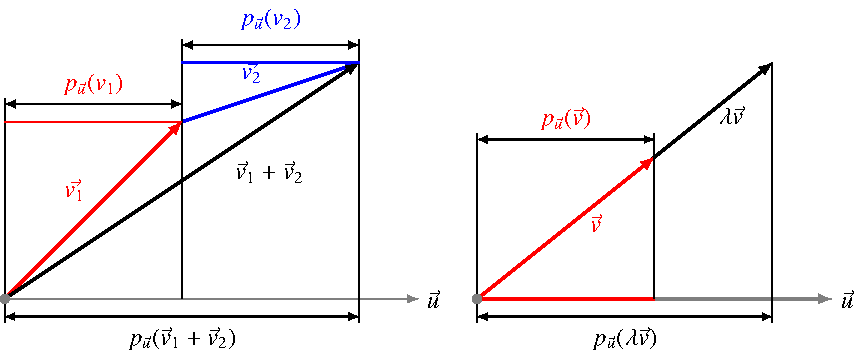
\includegraphics{4/images/linearitaet.pdf}
\caption{Die Projektionsabbilung
$\vec{v}\mapsto p_{\vec{u}}(\vec{v})$
ist linear. Die linke Graphik zeigt
$p_{\vec{u}}(\vec{v}_1+\vec{v}_2)
=
p_{\vec{u}}(\vec{v}_1)+p_{\vec{u}}(\vec{v}_2)$,
die rechte ist der Strahlensatz und zeigt
$p_{\vec{u}}(\lambda\vec{v})=\lambda p_{\vec{u}}(\vec{v})$.
\label{projektionlinearitaet}}
\end{figure}
Immerhin ist $p_{\vec u}(\vec v)$ linear in $\vec v$, wie man
sich mit der Abbildung~\ref{projektionlinearitaet}
sofort überzeugen kann, es ist also
\begin{align*}
p_{\vec u}(\vec v_1+\vec v_2)&=p_{\vec u}(\vec v_1)+p_{\vec u}(\vec v_2)\\
p_{\vec u}(\lambda \vec v)&=\lambda p_{\vec u}(\vec v).
\end{align*}

\subsection{Skalarprodukt}
\index{Skalarprodukt}
\begin{figure}
\begin{center}
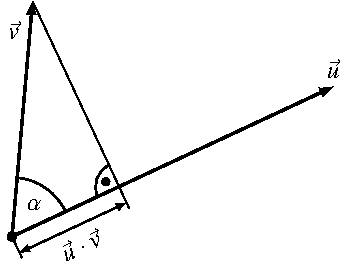
\includegraphics{4/images/skalarprodukt.pdf}
\end{center}
\caption{Skalarprodukt $\vec u\cdot \vec v$ des Einheitsvektors $\vec u$
und des Vektors $\vec v$ mit Zwischenwinkel
$\alpha$.\label{image-skalarprodukt}}
\end{figure}
Gesucht ist daher eine Konstruktion, welche immer noch linear ist,
aber auch symmetrisch in $\vec u$ und $\vec v$.
Die Formel (\ref{zwischenwinkel}) deutet auch an, wie dies erreicht
werden kann.
Der Zwischenwinkel kann natürlich auch berechnet werden,
indem die beiden Vektoren vertauscht werden:
\[
\cos \alpha
=
\frac{p_{\vec u}(\vec v)}{p_{\vec v}(\vec v)}
=
\frac{p_{\vec v}(\vec u)}{p_{\vec u}(\vec u)}
\]
Multipliziert man diese Gleichung mit
$
p_{\vec u}(\vec u)
p_{\vec v}(\vec v)
$, erhält man
\[
\vec u\cdot\vec v
=
p_{\vec u}(\vec u)
p_{\vec v}(\vec v)
\cos\alpha =
p_{\vec u}(\vec u)p_{\vec u}(\vec v)
=
p_{\vec v}(\vec v)p_{\vec v}(\vec u),
\]
was offenbar symmetrisch in $\vec u$ und $\vec v$ ist.

\begin{definition}Das Skalarprodukt zweier Vektoren $\vec u$ und
$\vec v$ ist
\[
\vec u\cdot\vec v
=
p_{\vec u}(\vec u)
p_{\vec v}(\vec v)
\cos\alpha.
\]
\end{definition}
Diese Grösse ist linear in $\vec u$ und linear in $\vec v$, und man kann
daraus $p_{\vec u}(\vec v)$ mittels
\[
p_{\vec u}(\vec v)
=
\frac{p_{\vec u}(\vec v)p_{\vec u}(\vec u)}{p_{\vec u}(\vec u)}
=
\frac{\vec u\cdot\vec v}{\sqrt{p_{\vec u}(\vec u)^2}}
=
\frac{\vec u\cdot\vec v}{\sqrt{\vec u\cdot \vec u}}
\]
wieder zurückgewinnen.

\begin{satz}
Seien $\vec u$ und $\vec v$ zwei Vektoren, dann ist
\[
|\vec u|=p_{\vec u}(\vec u)=\sqrt{\vec u\cdot\vec u}
\]
die Länge des Vektors, und für den Zwischenwinkel $\alpha$ gilt
\[
|\vec u|\,|\vec v|\cos\alpha=\vec u\cdot\vec v
\]
Zwei vom Nullvektor verschiedene Vektoren  stehen genau dann senkrecht
aufeinander, wenn $\vec u\cdot\vec v=0$.
Die Projektion $\vec v_{\|}$ von $\vec v$ auf $\vec u$ ist
\[
\vec v_{\|}=\frac{\vec v\cdot\vec u}{\vec u\cdot\vec u}\vec u.
\]
Ist $\vec u$ ein Einheitsvektor, dann ist $\vec v_{\|}=(\vec v\cdot \vec u)\vec u$.
\end{satz}
\index{Zwischenwinkel}

\subsection{Skalarprodukt und Standardbasis}
Zur praktischen Berechnung des Skalarproduktes benötigen wir
eine Formel, die das Skalarprodukt aus den Vektorkomponenten
berechnet.
Schreibt man
\[
\vec u=\begin{pmatrix}u_1\\u_2\\u_3\end{pmatrix}
=u_1\vec e_1+u_2\vec e_2+u_3\vec e_3
,
\qquad
\vec v=\begin{pmatrix}v_1\\v_2\\v_3\end{pmatrix}
=v_1\vec e_1+v_2\vec e_2+v_3\vec e_3
\]
dann kann das Skalarprodukt mit der Linearität berechnet werden:
\begin{align*}
\vec u\cdot\vec v
&=
(u_1\vec e_1+u_2\vec e_2+u_3\vec e_3)\cdot
(v_1\vec e_1+v_2\vec e_2+v_3\vec e_3)
\\
&=
u_1v_1\vec e_1\cdot\vec e_1+
u_1v_2\vec e_1\cdot\vec e_2+
u_1v_3\vec e_1\cdot\vec e_3\\
&\qquad +
u_2v_1\vec e_2\cdot\vec e_1+
u_2v_2\vec e_2\cdot\vec e_2+
u_2v_3\vec e_2\cdot\vec e_3\\
&\qquad+
u_3v_1\vec e_3\cdot\vec e_1+
u_3v_2\vec e_3\cdot\vec e_2+
u_3v_3\vec e_3\cdot\vec e_3
\end{align*}
Die Skalarprodukte von aufeinander senkrecht stehenden Vektoren
verschwinden, es bleiben nur die Termen mit $\vec e_i\cdot\vec e_i$,
das Skalarprodukt eines Vektors mit sich selbst ist das Quadrat
der Länge, also $\vec e_i\cdot \vec e_i=1$ und so erhalten wir den
Satz
\begin{satz}
Das Skalarprodukt zweier Vektoren
\[
\vec u=\begin{pmatrix}u_1\\u_2\\u_3\end{pmatrix},
\qquad
\vec v=\begin{pmatrix}v_1\\v_2\\v_3\end{pmatrix}
\]
ist
\[
\vec u\cdot\vec v
=
u_1v_1+u_2v_2+u_3v_3.
\]
\end{satz}

\begin{beispiel}
Berechne die Länge und den Zwischenwinkel der Vektoren
\begin{align*}
\vec a&= \begin{pmatrix} 3\\12\\ 4 \end{pmatrix},
&
\vec b&= \begin{pmatrix}2\\3\\6\end{pmatrix}.
\end{align*}

\smallskip

{\parindent 0pt Die} Länge der Vektoren ist
\begin{align*}
|\vec a|
&
=\sqrt{\vec a\cdot \vec a}
&
|\vec b|
&
=\sqrt{\vec b\cdot \vec b}
\\
&=\sqrt{9+144+16}
&
&=\sqrt{4+9+36}
\\
&=\sqrt{169}=13
&
&
=\sqrt{49}=7
\end{align*}
Damit kann man jetzt auch den Zwischenwinkel berechnen
\begin{align*}
\cos\alpha&= \frac{\vec a\cdot \vec b}{|\vec a|\;|\vec b|}
=
\frac{6+36+24}{13\cdot 7}=\frac{66}{91}=0.72527
\\
\alpha&=43.51^\circ
\end{align*}
\end{beispiel}
Häufig braucht man zu einem Vektor einen Vektor mit gleicher Richtung,
aber Einheitslänge.
Wir verwenden die Schreibweise
\[
\vec{v}^0 = \frac{\vec{v}}{|\vec{v}|}
\]
für den zum Vektor $\vec{v}$ gehörigen Einheitsvektor.

%\subsection{Ebenen}
%\begin{figure}
%\begin{center}
%\includegraphics{images/s-3}
%\end{center}
%\caption{Ebene in Normalenform\label{image-normalenform}}
%\end{figure}
%Das Skalarprodukt gibt uns eine neue Möglichkeit, Ebenen zu
%beschreiben.
%Eine Ebene durch den Punkt $P$ senkrecht auf den Vektor
%$\vec n$ besteht genau aus jenen Punkten $Q$, für die der Vektor
%$\overset{\rightarrow}{PQ}$ auf $\vec n$ senkrecht steht
%(Abbildung~\ref{image-normalenform}).
%Mit dem Skalarprodukt
%ausgedrückt: Die Menge der Ortsvektoren der Punkte einer Ebene durch $P$ mit
%\index{Normale}
%Normale $\vec n$ ist
%\[
%\{\vec r\;|\;(\vec r-\vec p)\cdot \vec n=0\}
%\]
%Multipliziert man die Gleichung aus, erhält man
%\begin{align*}
%\left(
%\begin{pmatrix}x\\y\\z\end{pmatrix}
%-\begin{pmatrix}p_1\\p_2\\p_3\end{pmatrix}\right)\cdot
%\begin{pmatrix}n_1\\n_2\\n_3\end{pmatrix}&=0
%\\
%(x-p_1)n_1+(y-p_2)n_2+(z-p_3)n_3&=0
%\\
%n_1x+n_2y+n_3z&=p_1n_1+p_2n_2+p_3n_3
%\end{align*}
%Diese Form der Ebenengleichung, in der $\vec n$ ein Einheitsnormalenvektor ist,
%heisst auch {\em Hessesche Normalform}.
%\index{Normalenform}
%\index{Hessesche Normalform}
%
%\begin{satz}
%Ist $\vec n$ ein Einheitsvektor, dann ist
%\[
%d=(\vec r-\vec p_0)\cdot \vec n
%\]
%der Abstand des Punktes mit dem Ortsvektor $\vec r$ von der Ebene durch
%den Punkt mit Ortsvektor $\vec p_0$ und Normalen $\vec n$.
%In Koordinaten:
%\[
%d=n_xx+n_yy+n_zz-\vec p_0\cdot\vec n
%\]
%\end{satz}
%\begin{proof}[Beweis]
%$(\vec r-\vec p)\cdot \vec n$ ist die Länge der Projektion des Vektors
%$\vec r -\vec p$ auf den Normalenvektor $\vec n$, also genau der behauptete
%Abstand.
%\end{proof}
%
%\begin{beispiel}
%Man finde die Normalenform der Ebenengleichung (\ref{beispielebene}) auf
%Seite~\pageref{beispielebene},
%und berechne den Abstand des Punktes $(1,1,1)$ von der Ebene.
%
%\medskip
%
%{\parindent 0pt Die} Lösung vollzieht sich in folgenden Schritten:
%\begin{compactenum}
%\item Bestimme die Normale der Ebene.
%\item Schreibe die Gleichung der Ebene in Normalenform.
%\item Bringe die Normalenform in Hessesche Normalform.
%\item Berechne den Abstand des Punktes $(1,1,1)$.
%\end{compactenum}
%Gesucht ist ein Vektor $\vec n$, der auf beiden
%Richtungsvektoren senkrecht steht, also
%\begin{equation}
%\begin{pmatrix}n_1\\n_2\\n_3\end{pmatrix}
%\cdot
%\begin{pmatrix}2\\2\\-2\end{pmatrix}
%=0,
%\qquad
%\begin{pmatrix}n_1\\n_2\\n_3\end{pmatrix}
%\cdot
%\begin{pmatrix}3\\-3\\-1\end{pmatrix}
%=0
%\label{gleichungen-fuer-normale}
%\end{equation}
%Dies ist gleichbedeutend mit dem Gleichungssystem
%\[
%\begin{pmatrix}
%2&2&-2\\
%3&-3&-1
%\end{pmatrix}
%\begin{pmatrix}n_1\\n_2\\n_3\end{pmatrix}
%=\begin{pmatrix}0\\0 \end{pmatrix}
%\]
%Der Gauss-Algorithmus liefert
%\begin{align*}
%\begin{tabular}{|>{$}c<{$}>{$}c<{$}>{$}c<{$}|}
%\hline
%2%
%\begin{picture}(0,0)
%\color{red}\put(-3,4){\circle{12}}
%\end{picture}%
%&2&-2\\
%3%
%\begin{picture}(0,0)%
%\color{blue}\drawline(-8,-2)(-8,10)(2,10)(2,-2)
%\end{picture}%
%&-3&-1\\
%\hline
%\end{tabular}
%&\rightarrow
%\begin{tabular}{|>{$}c<{$}>{$}c<{$}>{$}c<{$}|}
%\hline
%1&1&-1\\
%0&-6%
%\begin{picture}(0,0)%
%\color{red}\put(-7,4){\circle{15}}
%\end{picture}%
%&2\\
%\hline
%\end{tabular}
%\rightarrow
%\begin{tabular}{|>{$}c<{$}>{$}c<{$}>{$}c<{$}|}
%\hline
%1&1%
%\begin{picture}(0,0)
%\color{blue}\drawline(-8,10)(-8,-2)(2,-2)(2,10)
%\end{picture}%
%&-1\\
%0&1&-\frac13\\
%\hline
%\end{tabular}
%\rightarrow
%\begin{tabular}{|>{$}c<{$}>{$}c<{$}>{$}c<{$}|}
%\hline
%1&0&-\frac23\\
%0&1&-\frac13\\
%\hline
%\end{tabular}
%\end{align*}
%Die Komponente $n_3$ ist frei wählbar, wir setzen $n_3=3$, und bekommen
%$n_1=2$ und $n_2=1$.
%Tatsächlich ist
%\begin{align*}
%\begin{pmatrix}2\\1\\3\end{pmatrix}
%\cdot
%\begin{pmatrix}2\\2\\-2\end{pmatrix}
%&=4+2-6=0
%&
%\begin{pmatrix}2\\1\\3\end{pmatrix}
%\cdot
%\begin{pmatrix}3\\-3\\-1\end{pmatrix}
%&=6-3-3=0.
%\end{align*}
%Damit ist die Normalenform der Ebenengleichung
%\begin{align}
%\begin{pmatrix}2\\1\\3\end{pmatrix}\cdot\left(
%\begin{pmatrix}x\\y\\z\end{pmatrix} - \begin{pmatrix}1\\2\\1\end{pmatrix}
%\right)&=0\notag\\
%\Rightarrow\qquad
%2x+y+3z&=7\label{normalenform}
%\end{align}
%Diese Form ist zwar eine Normalenform, aber noch nicht die Hessesche
%Normalform, da man für diesen Zweck einen Einheitsvektor als
%Normalenvektor verwenden muss.
%Unser Normalenvektor hat aber die Länge $|\vec n|=\sqrt{14}$.
%Dividieren wir die Gleichung (\ref{normalenform})
%durch $\sqrt{14}$, erhalten wir die Hessesche Normalform:
%\begin{equation}
%d=\frac{2}{\sqrt{14}}x+\frac{1}{\sqrt{14}}y+\frac{3}{\sqrt{14}}z-\frac{7}{\sqrt{14}}.
%\label{hnf}
%\end{equation}
%Die Hessesche Normalform berechnet den Abstand eines Punktes von der
%Ebene.
%Man muss jetzt also nur noch den Punkt $(1,1,1)$ in die  Gleichung
%(\ref{hnf}) einsetzen:
%\[
%d = (2+1+3-7)/\sqrt{14}=-1/\sqrt{14}=-0.26726,
%\]
%der gesuchte Abstand ist also $d=0.26726$.
%\end{beispiel}
%
%\subsection{Spiegelung\label{spiegelung}}
%\begin{figure}
%\begin{center}
%\includegraphics{images/s-4}
%\end{center}
%\caption{Spiegelung eines Vektors $\vec v$ an der Ebene senkrecht auf $\vec n$.
%\label{image-spiegelung}}
%\end{figure}
%Da man mit dem Skalarprodukt senkrechte Projektionen berechnen kann,
%muss es auch möglich sein, die Spiegelung eines Vektors $\vec v$
%an einer Ebene mit Normale $\vec n$ zu berechnen ($|\vec n|=1$).
%Dazu zerlegt man den Vektor $\vec v$ in eine Komponente $\vec v_{\|}$
%parallel zur Ebene und eine Komponenten $\vec v_{\perp}$ senkrecht dazu,
%also $\vec v=\vec v_{\|}+\vec v_{\perp}$ (Abbildung~\ref{image-spiegelung}).
%Die senkrechte Komponente
%ist im wesentlichen die Projektion von $\vec v$ auf $\vec n$:
%\[
%\vec v_{\perp}=
%(\vec v\cdot\vec n)\vec n
%.
%\]
%Die parallele Komponente ist der Rest:
%\[
%\vec v_{\|}=\vec v -\vec v_{\perp}=
%\vec v-(\vec v\cdot\vec n)\vec n
%,
%\]
%Beim gespiegelten Vektor zeigt die senkrechte Komponente in die
%entgegengesetzte Richtung:
%\begin{equation}
%\vec v_{\text{gespiegelt}}=
%\vec v_{\|}-\vec v_{\perp}
%=
%\vec v-(\vec v\cdot\vec n)\vec n
%-
%(\vec v\cdot\vec n)\vec n
%=\vec v-2(\vec v\cdot\vec n)\vec n.
%\label{equation:spiegelung}
%\end{equation}
%
%\begin{beispiel}
%Man spiegle den Vektor $\vec a$ an der Ebene mit der Normalen $\vec n$,
%\[
%\vec a=\begin{pmatrix}1\\2\\3\end{pmatrix},
%\qquad
%\vec n=\begin{pmatrix}1\\1\\1\end{pmatrix}
%\]
%
%\smallskip
%
%{\parindent 0pt Zunächst stellen wir fest,} dass $\vec n$ noch
%kein Einheitsvektor ist, dass wir stattdessen $\vec n_0=\vec n/\sqrt{3}$
%verwenden müssen.
%Damit kann $\vec a$ jetzt die parallelen und orthogonalen
%Komponenten zerlegt werden:
%\[
%\vec a_{\perp}=(\vec a\cdot\vec n_0)\vec n_0
%=\frac1{\sqrt{3}} (1+2+3)\frac1{\sqrt{3}}\begin{pmatrix}1\\1\\1\end{pmatrix}
%=\begin{pmatrix}2\\2\\2\end{pmatrix},
%\quad
%\vec a_{\|}=\begin{pmatrix} -1\\0\\1 \end{pmatrix}.
%\]
%Nach Formel (\ref{equation:spiegelung}) ist
%\[
%\vec a'=\vec a_{\|}-\vec a_{\perp}
%=
%\begin{pmatrix}-1\\0\\1\end{pmatrix}-\begin{pmatrix}2\\2\\2\end{pmatrix}
%=\begin{pmatrix}-3\\-2\\-1\end{pmatrix}.
%\]
%der gespiegelt Vektor.
%\end{beispiel}

%\subsection{Orthonormalbasis}
%Die Vektoren $\vec e_i$ stehen senkrecht aufeinander und haben
%Länge $1$.
%Der Vektor
%\[
%\vec v
%=
%\begin{pmatrix}v_1\\v_2\\v_3\end{pmatrix}
%\]
%lässt sich mit Hilfe des Skalarproduktes als Summe von Vielfachen
%der Vektoren $\vec e_i$ schreiben.
%Es ist nämlich $v_i=\vec v\cdot\vec e_i$, also
%\[
%\vec v
%=
%\begin{pmatrix}v_1\\v_2\\v_3\end{pmatrix}
%=
%v_1\vec e_1
%+
%v_2\vec e_2
%+
%v_3\vec e_3
%=
%(\vec v\cdot \vec e_1)\vec e_1
%+
%(\vec v\cdot \vec e_2)\vec e_2
%+
%(\vec v\cdot \vec e_3)\vec e_3
%\]
%Dies funktioniert aber nicht nur für die Vektoren $\vec e_i$.
%Seien $\vec b_1$, $\vec b_2$ und $\vec b_3$ drei aufeinander senkrecht
%stehende Vektoren der Länge $1$.
%Mit dem Skalarprodukt kann man dies durch
%\[
%\vec b_i\cdot\vec b_j=\begin{cases}
%0&\qquad i\ne j\\
%1&\qquad i=j
%\end{cases}
%\]
%ausdrücken.
%Versucht man den den Vektor $\vec v$ als Linearkombination
%der Vektoren $\vec b_i$ zu schreiben, also
%\[
%\vec v
%=
%v_1'\vec b_1
%+
%v_2'\vec b_2
%+
%v_3'\vec b_3
%\]
%Berechnet man jetzt das Skalarprodukt von $\vec v$ mit $\vec b_i$,
%findet man
%\begin{align*}
%\vec v\cdot \vec b_i
%&=
%(
%v_1'\vec b_1
%+
%v_2'\vec b_2
%+
%v_3'\vec b_3
%)\cdot
%\vec b_i
%\\
%&=
%v_1'\vec b_1\cdot\vec b_i
%+
%v_2'\vec b_2\cdot\vec b_i
%+
%v_3'\vec b_3\cdot\vec b_i
%\\
%&=v_i'
%\end{align*}
%weil alle Skalarprodukte verschwinden ausser zwischen
%zwei gleichen Vektoren.
%
%\begin{definition} Die Koeffizienten der Einheitsmatrix
%\[
%\delta_{ij}=
%\begin{cases}
%0&\qquad i\ne j\\
%1&\qquad i=j
%\end{cases}
%\]
%heisst {\em Kronecker-Delta}.
%\end{definition}
%
%\begin{definition}
%$n$ Vektoren $\vec b_i$ heissen orthonormiert, wenn gilt
%\[
%\vec b_i\cdot\vec b_j=\delta_{ij}.
%\]
%\end{definition}
%
%\begin{satz}
%Sind die Vektoren $\vec b_i$ orthonormiert, dann kann man jeden
%Vektor $\vec v$ als Linearkombination der Vektoren $\vec b_i$
%\[
%\vec v=
%(\vec v\cdot\vec b_1)\vec b_1
%+
%(\vec v\cdot\vec b_2)\vec b_2
%+
%(\vec v\cdot\vec b_3)\vec b_3
%\]
%schreiben.
%Diese Darstellung ist eindeutig.
%\end{satz}
%
%\begin{proof}[Beweis]
%Es ist nur noch zu beweisen, dass es nur eine solche Darstellung als
%Linearkombination gibt.
%Gäbe es zwei Darstellungen, also
%\begin{align*}
%\vec v
%&=
%v_1'\vec b_1+
%v_2'\vec b_2+
%v_3'\vec b_3\\
%&=
%v_1''\vec b_1+
%v_2''\vec b_2+
%v_3''\vec b_3,
%\end{align*}
%können wir die Differenz bilden:
%\[
%0=
%(v_1'-v_1'')\vec b_1
%+
%(v_2'-v_2'')\vec b_2
%+
%(v_3'-v_3'')\vec b_3
%\]
%Das Skalarprodukt mit $b_i$ ergibt dann
%\[
%0=(v_i'-v_i'')\quad\Rightarrow\quad v_i'=v_i''.
%\]
%Da wir $i$ beliebig wählen können folgt, dass die
%Koeffizienten $v_i'$ und $v_i''$ übereinstimmen.
%\end{proof}
%
%%\subsection{Verallgemeinertes Skalarprodukt}
%
%%\begin{definition}
%%Ein symmetrische Matrix $g_{ij}$ definiert ein allgemeines Skalarprodukt
%%$$g(x,y)=\sum_{i,j=1}^ng_{ij}x_iy_i$$
%%der Vektoren
%%$$x=\begin{pmatrix}x_1\\\vdots\\x_n\end{pmatrix}\qquad\text{und}
%%\qquad y=\begin{pmatrix}y_1\\\vdots\\y_n\end{pmatrix}.$$
%%\end{definition}
%%Das zu Beginn dieses Abschnitts definiert Skalarprodukt ist ein
%%verallgemeinertes Skalarprodukt mit der Matrix $I$.
%
%\subsection{Orthonormalisierung}
%Für orthonormierte Vektoren ist es besonders einfach, eine Darstellung
%eines beliebigen Vektors als Linearkombination zu finden.
%Es ist daher sicher nützlich, aus einer Menge von Vektoren
%$\{\vec a_1,\vec a_2,\vec a_3\}$
%eine neue Menge von Vektoren zu konstruieren, die sich von der gegeben
%möglichst wenig
%unterscheidet, aber dennoch aus orthonormierten Vektoren besteht.
%
%\begin{satz}[Gram-Schmidt]
%\label{satz-gram-schmidt}
%Seien $\{\vec a_1,\vec a_2,\vec a_3\}$ linear unabhängige Vektoren.
%Dann gibt es orthonormierte Vektoren $\{\vec b_1,\vec b_2,\vec b_3\}$ so,
%dass $b_k$ aus $a_1,\dots,a_k$ linear kombiniert werden kann, für jedes $k$.
%Die $b_i$ lassen sich wie folgt berechnen
%\begin{align*}
%\vec b_1&=\frac1{|\vec a_1|}a_1\\
%\vec b_2&=
%\frac{
%\vec a_2-(\vec a_2\cdot \vec b_1)\vec b_1
%}{
%|\vec a_2-(\vec a_2\cdot \vec b_1)\vec b_1|
%}
%\\
%\vec b_3
%&=
%\frac{
%\vec a_3-(\vec a_3\cdot \vec b_1)\vec b_1-(\vec a_3\cdot\vec b_2)\vec b_2
%}{
%|
%\vec a_3-(\vec a_3\cdot \vec b_1)\vec b_1-(\vec a_3\cdot\vec b_2)\vec b_2
%|
%}
%\\
%&\phantom{=}\vdots\\
%\vec b_k&=\frac{\vec a_k-(\vec a_k\cdot \vec b_1)\vec b_1-(\vec a_k\cdot \vec b_2)\vec b_2-\dots-(\vec a_k\cdot \vec b_{k-1})\vec b_{k-1}}{|\vec a_k-(\vec a_k\cdot \vec b_1)\vec b_1-(\vec a_k\cdot \vec b_2)\vec b_2-\dots-(\vec a_k\cdot \vec b_{k-1})\vec b_{k-1}|}
%\end{align*}
%Das Verfahren lässt sich offenbar auf eine beliebige Zahl linear
%unabhängiger $n$-dimensionaler Vektoren verallgemeinern.
%\end{satz}
%
%Auf die Reihenfolge der Vektoren kommt es entscheidend an, wie die
%folgenden zwei Beispiele zeigen
%\begin{beispiel}
%Die Vektoren
%\[
%\vec a_1=\begin{pmatrix}1\\0\\0\end{pmatrix},\qquad
%\vec a_2=\begin{pmatrix}1\\1\\0\end{pmatrix},\qquad
%\vec a_3=\begin{pmatrix}1\\1\\1\end{pmatrix}
%\]
%sind zu orthonormieren.
%
%Die Formeln aus Satz~\ref{satz-gram-schmidt} liefern folgende Vektoren:
%\begin{align*}
%\vec b_1&=\frac{\vec a_1}{|\vec a_1|}=\begin{pmatrix}1\\0\\0\end{pmatrix}\\
%\vec b_2&=
%\frac{
%\vec a_2-(\vec a_2\cdot \vec b_1)\vec b_1
%}{
%|\vec a_2-(\vec a_2\cdot \vec b_1)\vec b_1|
%}
%=
%\frac{
%\begin{pmatrix}1\\1\\0\end{pmatrix}-1\cdot\begin{pmatrix}1\\0\\0\end{pmatrix}
%}{\dots}=\begin{pmatrix}0\\1\\0\end{pmatrix}\\
%\\
%\vec b_3&=
%\frac{\vec a_3 -(\vec a_3\cdot \vec b_1)\vec b_1-(\vec a_3\cdot\vec b_2)\vec b_2}{\dots}
%=\frac{\begin{pmatrix}1\\1\\1\end{pmatrix}-1\cdot \begin{pmatrix}1\\0\\0\end{pmatrix}-1\cdot\begin{pmatrix}0\\1\\0\end{pmatrix}
%}{\dots}=\begin{pmatrix}0\\0\\1\end{pmatrix}
%\end{align*}
%Man findet also genau die Vektoren der Standardbasis.
%\end{beispiel}
%
%\begin{beispiel}
%Die Vektoren
%\[
%\vec a_1=\begin{pmatrix}1\\0\\0\end{pmatrix},\qquad
%\vec a_2=\begin{pmatrix}1\\1\\1\end{pmatrix},\qquad
%\vec a_3=\begin{pmatrix}1\\1\\0\end{pmatrix}
%\]
%sind zu orthonormieren.
%
%Dieses Beispiel unterscheidet sich vom vorangegangenen nur
%durch die Reihenfolge der Vektoren.
%Wieder können die Formeln von Satz~\ref{satz-gram-schmidt} angewandt werden:
%\begin{align*}
%\vec b_1&=\frac{\vec a_1}{|\vec a_1|}=\begin{pmatrix}1\\0\\0\end{pmatrix}
%\\
%\vec b_2
%&=
%\frac{\vec a_2-(\vec a_2\cdot \vec b_1)\vec b_1}{\dots}
%=
%\frac{\begin{pmatrix}1\\1\\1\end{pmatrix}-1\cdot\begin{pmatrix}1\\0\\0\end{pmatrix}}{\dots}=\frac1{\sqrt{2}}\begin{pmatrix}0\\1\\1\end{pmatrix}
%\\
%\vec b_3
%&=
%\frac{\vec a_3-(\vec a_3\cdot\vec b_1)\vec b_1-(\vec a_3\cdot\vec b_2)\vec b_2}{\dots}
%=\frac{\displaystyle\begin{pmatrix}1\\1\\0\end{pmatrix}-1\cdot\begin{pmatrix}1\\0\\0\end{pmatrix}-\frac1{\sqrt{2}}\cdot\frac1{\sqrt{2}}\begin{pmatrix}0\\1\\1\end{pmatrix} }{\cdots}
%=\frac{1}{\sqrt{2}}\begin{pmatrix}0\\1\\-1\end{pmatrix}.
%\end{align*}
%Die gefundenen Vektoren sind völlig verschiedenen von den Vektoren
%im vorangegangenen Beispiel.
%\end{beispiel}

%\subsection{Überbestimmte Gleichungssysteme -- ``Least Squares''\label{section-least-squares}}
%Bei einem überbestimmten Gleichungssystem, als einem Gleichungssystem
%mit mehr Gleichungen als Unbekannten, kann man im allgemeinen nicht davon
%ausgehen, dass es überhaupt eine Lösung gibt.
%Ein solches Gleichungssystem hat die Form
%\[
%A v= b,
%\]
%wobei $A$ eine Matrix ist, die mehr Zeilen als Spalten hat.
%In drei Dimensionen hat $v$ also zwei oder sogar nur eine Komponenten,
%die Menge aller möglichen Vektoren $Av$ ist also eine Ebene oder
%Gerade.
%
%\subsubsection{Lösung im Sinne kleinsten Abstandes}
%Das beste, was man erwarten kann, ist ein Vektor $v_0$ so, dass
%der Abstand des Punktes $ b$ von der Ebene (Gerade) bestehende
%aus allen $Av$ für $v=v_0$ am kleinsten wird.
%Dies geschieht
%natürlich genau dann, wenn der Differenzvektor $b-Av_0$ auf
%allen Vektoren von $Av$ senkrecht steht.
%
%Die Menge der Vektoren der Form $Av$ wird von den Spalten von $A$
%aufgespannt, es genügt also zu testen, ob $b-Av_0$ auf diesen
%Vektoren senkrecht steht.
%Dazu müssen die Skalarprodukte von
%Spalten von $A$ mit dem Vektor $b-Av_0$ verschwinden, oder
%\[
%A^t(b-Av_0)=0
%\quad
%\Rightarrow
%\quad
%A^tAv_0=A^tb
%\]
%wir haben also ein Gleichungssystem gefunden mit Matrix $A^tA$ und
%rechter Seite $A^tb$, welches als Lösung den gesuchten Vektor
%$v_0$ hat.
%$A^t$ hat so viele Zeilen wie $v$ Komponenten hat, also
%handelt es sich um ein Gleichungssystem mit gleich vielen Gleichungen
%wie Unbekannten, es wird im Allgemeinen eine eindeutig bestimmte
%Lösung haben.
%
%\begin{satz} Sei $A$ eine $n\times m$ Matrix und $b$ ein $n$-dimensionaler
%Vektor.
%Eine Lösung im Sinne minimaler quadrierter Abstände
%$
%(Av-b)\cdot(Av-b)
%$
%ist Lösung des Gleichungssystems
%\[
%A^tAv=A^tb
%\]
%mit $m$ Gleichungen und $m$ Unbekannten.
%\end{satz}
%
%\begin{beispiel}
%Man finden den Fusspunkt des Lotes vom Punkt $P=(9,10,7)$ auf die Ebene
%durch $O$, $A=(8,10,10)$ und $B=(9,13,12)$.
%
%Der Fusspunkt des Lotes ist der Punkt der Ebene, der den geringsten
%Abstand zu $P$ hat.
%Die Ebenengleichung ist
%\[
%A\begin{pmatrix}s\\t\end{pmatrix}=
%\begin{pmatrix}
% 8& 9\\
%10&13\\
%10&12
%\end{pmatrix}
%\begin{pmatrix}s\\t\end{pmatrix}.
%\]
%Gesucht wird die ``beste Lösung'' von
%\[
%A\begin{pmatrix}s\\t\end{pmatrix}=\begin{pmatrix}9\\10\\7\end{pmatrix}=b
%\]
%Dazu muss zunächst die Matrix $A^tA$ und der Vektor $A^tb$
%berechnet werden.
%\[
%A^tA=\begin{pmatrix}
%264&322\\
%322&394
%\end{pmatrix}
%,\qquad
%A^tb=\begin{pmatrix}
%242\\295
%\end{pmatrix}.
%\]
%Daraus findet man die Lösung für $s$ und $t$ numerisch zu
%\[
%\begin{pmatrix}s\\t \end{pmatrix}
%=
%\begin{pmatrix}
%   1.07831\\
%  -0.13253
%\end{pmatrix}
%\]
%und durch Einsetzen in die Ebenengleichung den Ortsvektor des Fusspunktes
%\[
%\vec f = \begin{pmatrix}
%   7.4337\\
%   9.0602\\
%   9.1928
%\end{pmatrix}
%\]
%Man kann dieses Resultat dadurch kontrollieren, dass man nachrechnet, ob
%$\vec p-\vec f$ senkrecht auf beiden Richtungsvektoren der Ebene
%steht:
%\[
%(\vec p-\vec f)^tA=\begin{pmatrix}
%  -1.7451\cdot10^{-11}&  -2.1316\cdot 10^{-11}
%\end{pmatrix},
%\]
%im Rahmen der Rechengenauigkeit steht die Differenz also tatsächlich auf
%den Richtungsvektoren senkrecht.
%\end{beispiel}
%
%\subsubsection{``Alles in einem Schritt''}
%In Abschnitt \ref{section-vereinheitlichtes-verfahren} wurde gezeigt,
%wie man Schnittproblem mit nur einer Durchführung des Gauss-Algorithmus
%lösen konnte.
%Im soeben gelösten Problem musste man aber wieder
%in mehrere Schritten vorgehen.
%Zuerst wurden $s$ und $t$ bestimmt,
%und erst in einem zweiten Schritt konnte der Fusspunkt des Lotes
%berechnet werden.
%
%Natürlich ist das auch für dieses Problem möglich, man behandelt
%$x$, $y$ und $z$ einfach als zusätzliche Variablen, die als Koordinaten
%von $Av$ berechnet werden.
%Das Gauss-Tableau dazu ist
%\[
%\begin{tabular}{|>{$}c<{$}>{$}c<{$}>{$}c<{$}>{$}c<{$}|>{$}c<{$}|}
%\hline
%x&y&z&s\quad t&\\
%\hline
%1&0&0&        &0\\
%0&1&0&-A   &0\\
%0&0&1&        &0\\
%\hline
% & & &A^tA    &A^tb\\
%\hline
%\end{tabular}
%\]
%\begin{beispiel}
%Für das Zahlenbeispiel lautet dieses Gauss-Tableau:
%\[
%\begin{tabular}{|>{$}c<{$}>{$}c<{$}>{$}c<{$}>{$}c<{$}>{$}c<{$}|>{$}c<{$}|}
%\hline
%x&y&z&s  &  t&\\
%\hline
%1&0&0& -8& -9&0\\
%0&1&0&-10&-13&0\\
%0&0&1&-10&-12&0\\
%\hline
%0&0&0&264&322&242\\
%0&0&0&322&394&295\\
%\hline
%\end{tabular}
%\rightarrow
%\begin{tabular}{|>{$}c<{$}>{$}c<{$}>{$}c<{$}>{$}c<{$}>{$}c<{$}|>{$}r<{$}|}
%\hline
%x&y&z&s  &  t&\\
%\hline
%1&0&0&0&0&7.4337\\
%0&1&0&0&0&9.0602\\
%0&0&1&0&0&9.1928\\
%\hline
%0&0&0&1&0&1.0783\\
%0&0&0&0&1&-0.1325\\
%\hline
%\end{tabular}
%\]
%Man erhält also genau die bereits früher gefundenen Lösungen.
%\end{beispiel}
%
